\documentclass{article}

\usepackage{amsmath}
\usepackage{amssymb}
\usepackage{graphicx}
\usepackage{subfigure}
\usepackage{enumerate}
\usepackage{tikz}
\usepackage{qtree}
\usepackage{clrscode3e}
\usepackage{hyperref}
\usepackage{bigstrut}

\pagestyle{plain}

\usepackage[left=3cm,top=2cm,right=3cm,nohead,nofoot]{geometry}

\begin{document}

\begin{center}
\bfseries 685.621 Algorithms for Data Science \\
Homework 3 \\
Assigned at the start of Module 6 \\
Due at the end of Module 8 - Tuesday March 23 (Midnight PST, 3AM EST)\\
Total Points $100/100$
\end{center}


Collaboration groups will be assigned on Tuesday march 2nd in Blackboard. Make sure your group starts one thread for the collaborative problems. You are required to participate in the collaborative problem and subproblem separately. Please do not directly post a complete solution, the goal is for the group to develop a solution after everyone has participated.\\

\begin{enumerate}

    %%%%%%%%%%%%%%%%%%%%%%%%% Problem 1 %%%%%%%%%%%%%%%%%%%%%%%%%%%%%%%%%%%%%%%
    \item \textbf{Problem 1}  \textbf{\emph{This is a Collaborative Problem}}\\
    30 Points Total 

In this problem, you will be developing pseudocode and implementing your development in Java, Matlab, Python or R for the Expectation Maximization method. 

  	\begin{enumerate}
		\item The development and implementation should be for a generic number of clusters, features and observations.
		\item Apply your implementation using the features generated from HW 2 for the numerical data set.
		\begin{enumerate}
			\item Use the top two ranked features.
			\item Create 4 clusters using the 4 numerical values that have the best separation.
			\item Display the 4 numerical values using 4 different colors for a good visual representation.
			\item Provide an analysis of your results, e.g., what is your observation of the results.
		\end{enumerate}
	\end{enumerate}

    \vspace{5mm}

        %%%%%%%%%%%%%%%%%%%%%%%%% Problem 2 %%%%%%%%%%%%%%%%%%%%%%%%%%%%%%%%%%%%%%%
    \item \textbf{Problem 2 - Chapter 1 and 2 [8]} \textbf{\emph{Note this is not Collaborative Problem}}\\
    10 Points Total\\
    
    Define in your own words the following terms: 
    \begin{enumerate}
		\item agent
		\item agent function
		\item agent program
		\item artificial intelligence
		\item autonomy
		\item goal-based agent
		\item intelligence
		\item learning agent
		\item logical reasoning
		\item model-based agent
		\item rationality 
		\item reflex agent
		\item utility-based agent
	\end{enumerate}
    
    \vspace{5mm}

   %%%%%%%%%%%%%%%%%%%%%%%%% Problem 3 %%%%%%%%%%%%%%%%%%%%%%%%%%%%%%%%%%%%%%%
    \item \textbf{Problem 3 - Chapter 2 [8]} \textbf{\emph{This is a Collaborative Problem}}\\
    30 Points Tota\\

	For your Tic-Tac-Toe implementation from PA1 add an agent to evaluate the board and the next best move.
	
	\begin{itemize}
		\item Best Move (Provided)
		\item (Completed from PA1) Implement a method that uses conditional statements to play against a user of your code. You must always check to see if your AI has a WIN and take that move, if not check to ensure your opponent does not have a WIN, if your opponent has a WIN possibility you must block your opponent. 
		\item Develop in pseudocode or code the agent of your choice (this is your algorithm you will need to provide the running time for).
		\item Implement the agent in your Tic-Tac-Toe game to make the next best move according to your intelligent agent.
		\item Provide the efficiency (running time) of your algorithm in $O$-notation.
		\item Provide the total running time of your algorithm in $T(n)$ as well as showing the cost at each line of code in your algorithm. 
	\end{itemize}

    \vspace{5mm}

   %%%%%%%%%%%%%%%%%%%%%%%%% Problem 4 %%%%%%%%%%%%%%%%%%%%%%%%%%%%%%%%%%%%%%%
    \item \textbf{Problem 4 } \\
    30 Points Total\\
    
The Parzen window algorithm density model is optimized by maximizing the likelihood of the training data with the use of a Gaussian window surrounding each input data point. In this problem the following is to be completed:\\
		\begin{enumerate}
			\item {[15 points]} \textbf{\emph{Note this is not Collaborative Problem}}\\
			Using the Gaussian kernel develop psuedo code to create a Parzen windowing system to accomplish the following steps:
				\begin{enumerate}
					\item Develop the ability to read in data $\textbf{x}_n$ with $n$ observations and $D$ dimensions (number of features).
					\item Develop the ability to randomly remove $20\%$ of the observations per class and assign the observations as test data with the remaining $80\%$ of the observations as training data.  
					\item Using the Gaussian kernel in Eq. 24 of the Machine Learning document to develop an algorithm to process an input observations and compare it with the training observations.
					\item Expand the development to handle multiple classes.
				\end{enumerate}
			\item {[10 points]} \textbf{\emph{Note this is not a Collaborative Problem}}
				\begin{enumerate}
					\item Calculate the running time of the system above in $O$-notation.
					\item Calculate the total running time of the above system as $T(n)$ with each line of pseudocode or code accounted for.
					\item How does the total running time $T(n)$ compare to the running time in $O$-notation?
				\end{enumerate}
			\item {[15 points]} \textbf{\emph{Note this is not a Collaborative Problem}}
				\begin{enumerate}
					\item Using all observations and the petal length from the Iris data replicate the subfigures in Figure 1.  
					\item Using all observations, the petal length and the petal width from the Iris data replicate the subfigures in Figure 2.  
				\end{enumerate}
		\end{enumerate}

\begin{figure}[htbp]
	\begin{center}
    		\subfigure[Gaussian Kernel with h = 0.1] {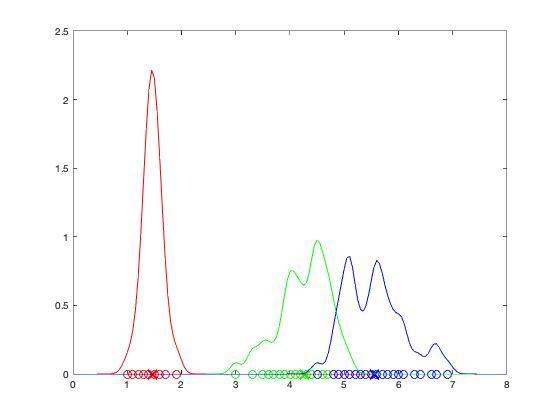
\includegraphics[width=7.6cm]  {gaussianIris0_1.jpg}  \label{fig:gaussianIris0_1}}\\
    		%\hspace{0.1pc}
		\subfigure[Gaussian Kernel with h = 0.25] {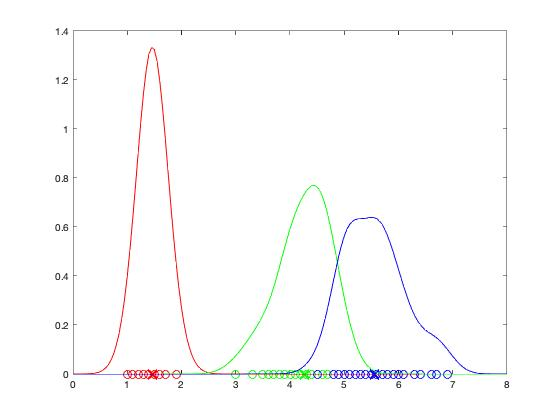
\includegraphics[width=7.6cm]  {gaussianIris0_25.jpg}  \label{fig:gaussianIris0_25}}
    		%\hspace{0.1pc}
		\subfigure[Gaussian Kernel with h = 0.5] {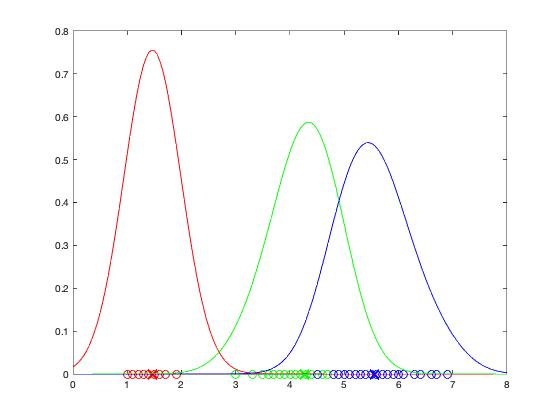
\includegraphics[width=7.6cm]  {gaussianIris0_5.jpg}  \label{fig:gaussianIris0_5}}
    		%\hspace{0.1pc}
    		\caption{Iris Data - Petal Length with Setosa in Red, Versicolor in Green and Virginica in Blue}
    		\label{fig:synthetic_data}
	\end{center}
\end{figure}

\begin{figure}[htbp]
	\begin{center}
    		\subfigure[Gaussian Kernel with h = 0.1] {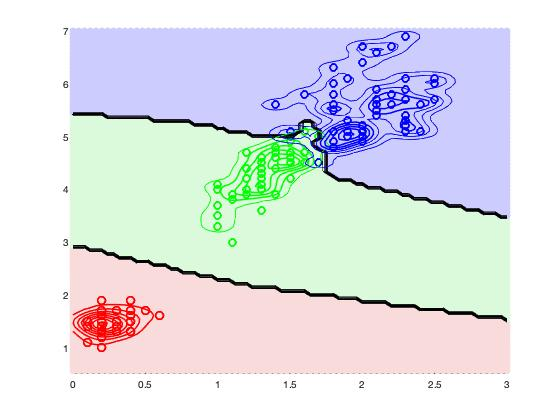
\includegraphics[width=7.6cm]  {gaussianIris2_0_1.jpg}  \label{fig:gaussianIris0_1}}\\
    		%\hspace{0.1pc}
		\subfigure[Gaussian Kernel with h = 0.25] {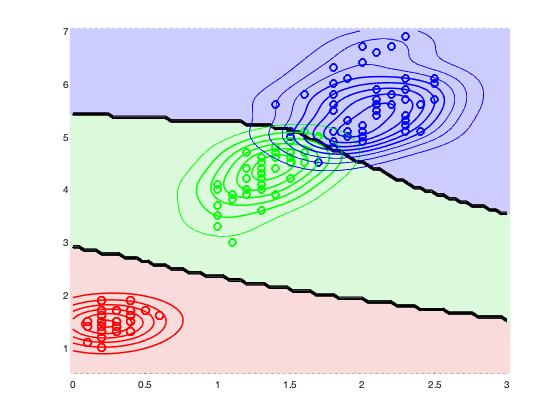
\includegraphics[width=7.6cm]  {gaussianIris2_0_25.jpg}  \label{fig:gaussianIris0_25}}
    		%\hspace{0.1pc}
		\subfigure[Gaussian Kernel with h = 0.5] {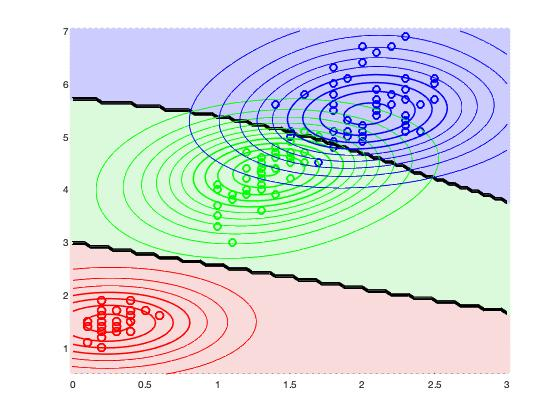
\includegraphics[width=7.6cm]  {gaussianIris2_0_5.jpg}  \label{fig:gaussianIris0_5}}
    		%\hspace{0.1pc}
    		\caption{Iris Data - Petal Length vs Petal Width with Setosa in Red, Versicolor in Green and Virginica in Blue}
    		\label{fig:synthetic_data}
	\end{center}
\end{figure}

    
    \vspace{5mm}
    
       %%%%%%%%%%%%%%%%%%%%%%%%% Problem 5 %%%%%%%%%%%%%%%%%%%%%%%%%%%%%%%%%%%%%%%

\textbf{References}

\begin{enumerate} 
	\item[{[1]}] Bishop, Christopher M., \textit{Neural Networks for pattern Recognition}, Oxford University Press, 1995 
	\item[{[2]}] Bishop, Christopher M., \textit{Pattern Recognition and Machine Learning}, Springer, 2006, \\
	https://www.microsoft.com/en-us/research/uploads/prod/2006/01/Bishop-Pattern-Recognition-and-Machine-Learning-2006.pdf
	\item[{[3]}] Duin, Robert P.W., Tax, David and Pekalska, Elzbieta, \textit{PRTools}, http://prtools.tudelft.nl/
	\item[{[4]}] Dempster, A. P., Laird, N. M. and Rubin, D. B., \textit{Maximum likelihood from incomplete data via the EM algorithm}, Journal of the Royal Statistical Society B, Volume 39, Number 1, pp.1–22, 1977
	\item[{[5]}] Franc, Vojtech and Hlavac, Vaclav, \textit{Statistical Pattern Recognition Toolbox}, \newline https://cmp.felk.cvut.cz/cmp/software/stprtool/index.html
	\item[{[6]}] Fukunaga, Keinosuke, \textit{Introduction to Statistical Pattern Recognition}, Academic Press, 1972 
	\item[{[7]}] Machine Learning at Waikato University, \textit{WEKA}, https://www.cs.waikato.ac.nz/~ml/index.html
	\item[{[8]}] Russell, S., and Norvig, P., \textit{Artificial Intelligence A Modern Approach}, $4^{th}$ Edition, Pearson, 2020
	\item[{[9]}] Tomasi, C., \textit{Estimating Gaussian Mixture Densities with EM – A Tutorial}, Duke University Course Notes, 2006, http://www.cs.duke.edu/courses/spring04/cps196.1/handouts/EM/tomasiEM.pdf, Retrieved Sept 2006
\end{enumerate}



\end{enumerate}
\end{document}
